\chapter{Results}\label{C:results} 
\section{Java}
The intent in analysing the Qualitas Corpus of Java code is to determine the extent to which developers are making use of Java's inbuilt language features and what developers are doing to work around these language features. Specifically, a Java developers' usage of class inheritance will represent them conforming to the classical inheritance model encouraged by the Java language. In contrast, instances of code which model call forwarding or call delegation will represent cases where the developer could have expressed themselves more concisely through other object inheritance models where delegation and forwarding are supported natively. The following patterns are used to identify instances of each model of reuse within the Java projects.


\begin{center}
	\captionof{table}{Java Patterns}
	\begin{tabular}{|p{5cm}|p{9cm}|}
		\hline
		
		\multicolumn{2}{|c|}{Java}                                                                   
		
		\\ \hline
		
		Forwarding                     & \code{anything name (anything)\{} \newline  \hphantom{----}\java{return identifier{[}.identifier{]}*.name(anything);} \newline
		\java{\}}  \\ 
		\hline
		
		Call Delegation                     & \code{anything name (anything) \{} \newline   \hphantom{----}\code{return identifier{[}.identifier{]}*.name(this);} \newline \code{\}}		
		\\ \hline
		
		Constructor Delegation & \code{anything anything = new anything ( this )}
		
		\\ \hline
		
		Inheritance                    & \code{class extends anything}

		\\ \hline
	\end{tabular}\newline\newline
\end{center}

The presence of two patterns representing delegation is because there are two main ways this behaviour can be represented in Java. The first, call delegation, is where an object passes itself as a parameter to some delegatee and has that delegatee perform some action on its behalf. The second, constructor delegation, is where a delegatee is constructed specifically for the instance of the delegator. This delegatee can then act on that constructor argument when its other methods are called.
\newline

Finding occurrences of classical inheritance in Java is as simple as looking for the extends keyword with a "grep" regular expression search. Finding examples of delegation and forwarding is more difficult and requires more information about the syntax tree of the program. To achieve this, each program of the corpus was passed through ANTLR which parses each file according to a Java grammar and constructs an abstract syntax tree which can then be traversed to search for relevant patterns.
\newline

The process for analysing a Java project follows a pipeline structure where each file is parsed and analysed in isolation. The resulting statistics of each file are then aggregated to form the overall statistics across the projects. This file isolation is important because the syntax trees produced by ANTLR consume large amounts of memory so it is not possible to hold all the Java files for a project in memory simultaneously.
\newline

\begin{center}
	\captionof{figure}{Java Analysis Pipeline}
	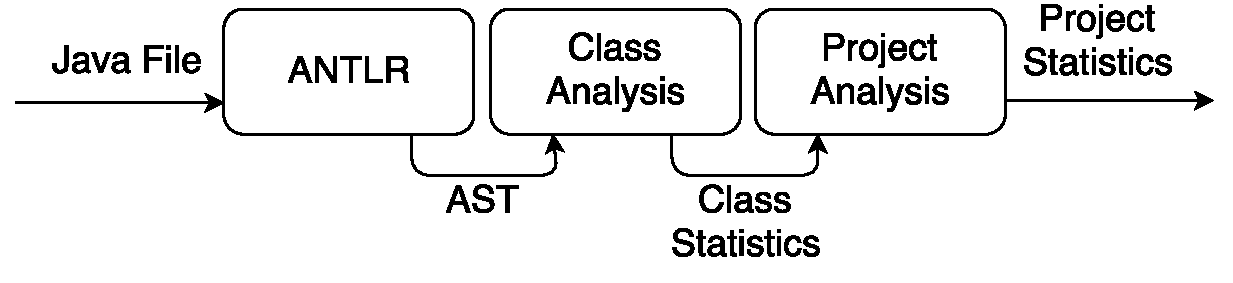
\includegraphics[scale=0.70]{AntlrPipeline.pdf}
\end{center}

The results are then aggregated to produce corpus level analysis which can be found in the following table:

\begin{center}
	\captionof{table}{Java Analysis Results}
	\begin{tabular}{|l|l|l|l|}
		\hline
		& Count  & \% of classes & \% of extended classes \\ \hline
		Total classes                                                                                   & 116427 &               &                        \\ \hline
		Classes extend another class                                                                    & 71203  & 61.16\%       &                        \\ \hline
		Classes are extended by another class                                                           & 20751  & 17.82\%       &                        \\ \hline
		Classes with forwarding                                                                         & 7087   & 6.09\%        &                        \\ \hline
		\begin{tabular}[c]{@{}l@{}}Classes with forwarding\\ that extend another class\end{tabular}     & 3381   & 2.90\%        &                        \\ \hline
		Classes with downcalls in constructors                                                          & 16101  & 13.83\%       &                        \\ \hline
		Classes storing this in constructors                                                            & 2392   & 2.05\%        &                        \\ \hline
		\begin{tabular}[c]{@{}l@{}}Classes with downcalls or\\ storing this in constructor\end{tabular} & 17099  & 14.69\%       &                        \\ \hline
		\begin{tabular}[c]{@{}l@{}}Extended classes with\\ downcalls in constructors\end{tabular}       & 1545   & 1.33\%        & 7.45\%                 \\ \hline
		\begin{tabular}[c]{@{}l@{}}Extended classes storing\\ this in constructors\end{tabular}         & 178    & 0.15\%        & 0.86\%                 \\ \hline
		Classes with delegation                                                                         & 5183   & 4.45\%        &                        \\ \hline
	\end{tabular}
\end{center}

\section{JavaScript}
In JavaScript, there are many ways developers make use of classical inheritance patterns despite the lack of native support in the language. This is largely a result of the numerous libraries which offer their own implementation of classical inheritance behaviour. Some examples of these patterns can be found in the following table:
\begin{center}
	\captionof{table}{JavaScript Patterns}
	\begin{tabular}{|p{5cm}|p{9cm}|}
		\hline
		\multicolumn{2}{|c|}{JavaScript}                                                                                                                                                                  \\ \hline
		Inheritance 1                  & \code{var a = function( b )\{    c.call ( this , d );\}}                                                                                      \\ \hline
		Inheritance 2                  & \code{function Bar( x , y )\{    Foo.call ( this , x ) ;\}}                                                                                 \\ \hline
		Inheritance 3                  & \code{Foo.prototype = object.create ( Bar.prototype )}                                                                                      \\ \hline
		Inheritance 4 - Node.js        & \code{var className = defineClass(...)}                                                                                                           \\ \hline
		Inheritance 5 - Node.js        & \code{ util.inherits(...)}                                                                                                                         \\ \hline
	\end{tabular}\newline\newline
\end{center}

The JavaScript analysis in this study makes extensive use of the prior work in developing the JSClassFinder application~\cite{JSClassFinder}. The aim here is to find the cases where JavaScript developers are choosing not to use the native delegation support of the language and are instead modelling their programs with classical inheritance structures. The important factor here is the Class Usage Ratio (CUR) of a JavaScript project as defined in \textit{Does JavaScript Software Embrace Classes?~\cite{JSClassFinder}}. Across a corpus of 50 JavaScript projects, the JSClassFinder returns interesting results about the prevalence of class usage in the language.
\begin{enumerate}
	\item The median CUR across the corpus was 0.15
	\item The upper quartile CUR across the corpus was 0.36
	\item The lower quartile CUR across the corpus was 0.005, which was heavily impacted by 13 systems which had a CUR of zero
\end{enumerate}
\section{Lua}
Table \ref{LuaResults} shows a variety of patterns often representative of class usage and the percentage of files in the corpus which exhibit one or more of those patterns.\newline

Often functions called class() will be created to encapsulate the \java{setmetatable()} logic which is used to create classes. It is also common to declare functions with the name "new" for use as constructors.

\begin{center}
	\captionof{table}{Lua Analysis Results}
	\label{LuaResults}
	\begin{tabular}{|l|l|l|l|}
		\hline
		Pattern                 & Test               & Result & Percentage \\ \hline
		= setmetatable()        &                    &        &            \\ \hline
		& Total matches      & 135    &            \\ \hline
		& Files with matches & 74     & 2.67\%     \\ \hline
		class(                  &                    &        &            \\ \hline
		& Total matches      & 487    &            \\ \hline
		& Files with matches & 380    & 13.69\%    \\ \hline
		function something.new( &                    &        &            \\ \hline
		& Total matches      & 31     &            \\ \hline
		& Files with matches & 30     & 1.08\%     \\ \hline
		Union of all three      &                    &        &            \\ \hline
		& Total matches      & 653    &            \\ \hline
		& Files with matches & 473    & 17.04\%    \\ \hline
	\end{tabular}
\end{center}{

\section{C\#}
C\# is a useful language to investigate because it requires use of the \cs{virtual} keyword to enable overriding of any given method. This is interesting because it makes it much more clear whether there could potentially be construction issues if we had a different way of initialising objects. When the \cs{virtual} keyword is required, the only method calls which could miss their intended target when used in a constructor are those which are explicitly labelled as \cs{virtual} dispatch calls.

\subsection{Results from GREP}
\begin{center}
	\captionof{table}{C\# Analysis Results}
	\label{CsResults}
	\begin{tabular}{|l|l|l|l|}
		\hline
		& Count   & Percent of files & Percent of methods \\ \hline
		Total projects                       & 25      &                  &                    \\ \hline
		Total C\# files                      & 73094   &                  &                    \\ \hline
		Total methods                        & 1415919 &                  &                    \\ \hline
		Files with methods                   & 67480   & 92.32\%          &                    \\ \hline
		Average methods per file             & 19.37   &                  &                    \\ \hline
		&         &                  &                    \\ \hline
		Total override methods               & 85347   &                  & 6.03\%             \\ \hline
		Files with override methods          & 18437   & 25.22\%          &                    \\ \hline
		Average override methods per file    & 1.17    &                  &                    \\ \hline
		&         &                  &                    \\ \hline
		Total virtual methods                & 27668   &                  & 1.95\%             \\ \hline
		Files with virtual methods           & 4553    & 6.23\%           &                    \\ \hline
		Average virtual methods per file     & 0.38    &                  &                    \\ \hline
		&         &                  &                    \\ \hline
		Total classes                        & 159680  &                  &                    \\ \hline
		Files with classes                   & 59488   & 81.39\%          &                    \\ \hline
		Average classes per file             & 2.18    &                  &                    \\ \hline
		&         &                  &                    \\ \hline
		Classes that extend                  & 50442   &                  &                    \\ \hline
		Files with classes that extend       & 30424   & 41.62\%          &                    \\ \hline
		Average classes that extend per file & 0.69    &                  &                    \\ \hline
		Percent of classes that extend       & 31.59\% &                  &                    \\ \hline
	\end{tabular}
\end{center}
Here, we find that just 1.95\% of all method declarations contain the \cs{virtual} keyword.
\newline\newline
\subsection{Results from ANTLR}
Projects: 15\newline
Files: 8154\newline
Classes: 15706\newline
Extending Classes: 7033\newline
Methods: 37745\newline
Virtual Methods: 5624\newline
Override Methods: 6229\newline
Classes with calls to local methods in constructors: 420\newline
Classes with calls to local virtual methods in constructors: 26\newline
Classes with calls to local override methods in constructors: 22\newline
Classes with calls to local abstract methods in constructors: 5\newline
Classes with calls to methods that couldn't be found in constructors: 189\newline